\section{Results \& Discussion}

\begin{figure}[h] %  figure placement: here, top, bottom, or page
    \centering
    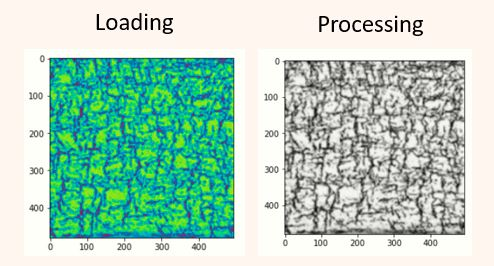
\includegraphics[width=4.5in]{Figures/4-Results/loading&processing.JPG}
    \caption{Image to be analysed, before and after processing.}
    \label{fig:limitationrhcf}
\end{figure}


\begin{figure}[h] %  figure placement: here, top, bottom, or page
    \centering
    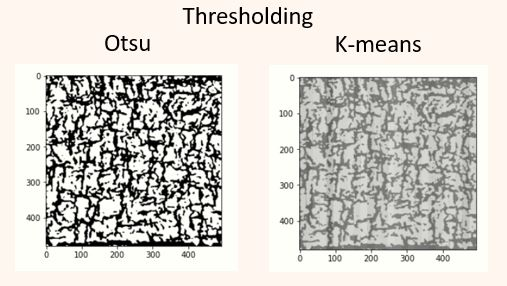
\includegraphics[width=4.5in]{Figures/4-Results/thresholding.JPG}
    \caption{Images after two different thresholds are applied: a) Otsu b) K-means.}
    \label{fig:limitationrhcf}
\end{figure}


\begin{figure}[h] %  figure placement: here, top, bottom, or page
    \centering
    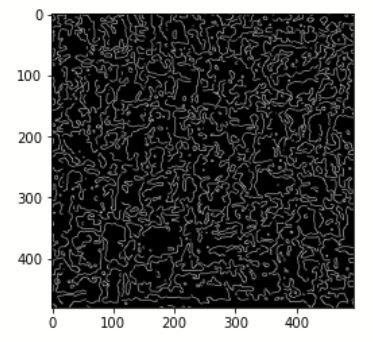
\includegraphics[width=2.5in]{Figures/4-Results/Otsu.JPG}
    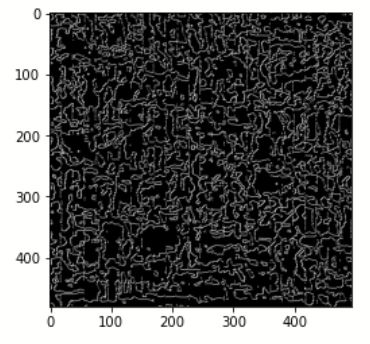
\includegraphics[width=2.5in]{Figures/4-Results/k-means.JPG}
    \caption{Connectivity of the images with a) Otsu threshold, b) K-means threshold.}
    \label{fig:limitationrhcf}
\end{figure}

